% 
%  chapter1.tex
%  ThesisISEL
%  
%  Created by Serge Lage on 2019/07/30.
%
% ================
% = Introduction =
% ================
\chapter{Server}
\label{cha:server}
This chapter explains the approach used to reach the second goal of this work. 

\section{Introduction} % (fold)
\label{sec:introduction}
Data mining is the process of discovering interesting and useful patterns and relationships in large volumes of data. The field combines tools from statistics and artificial intelligence (such as neural networks and machine learning) with database management to analyze large digital collections, known as data sets. Data mining is widely used in business (insurance, banking, retail), science research (astronomy, medicine), and government security (detection of criminals and terrorists) \cite{Okonkwo2011COMBATINGCA}. 

In this work it will be used the CRISP-DM (CRoss Industry Standard Process for Data Mining) methodology \cite{CRISPDM}.
The CRISP-DM project proposed a comprehensive process model for carrying out data mining projects. The process model is independent of both the industry sector and the technology used \cite{CRISPDM}. 
The CRISP-DM reference model for data mining provides an overview of the life cycle of a data
mining project. It contains the phases of a project, their respective tasks, and their outputs.
The life cycle of a data mining project is broken down in six phases which are shown in \ref{fig:crisp_dm}.
The sequence of the phases is not strict. The arrows indicate only the most important and frequent
dependencies between phases, but in a particular project, it depends on the outcome of each phase
which phase, or which particular task of a phase, has to be performed next.

\begin{figure}[H]
    \centering
    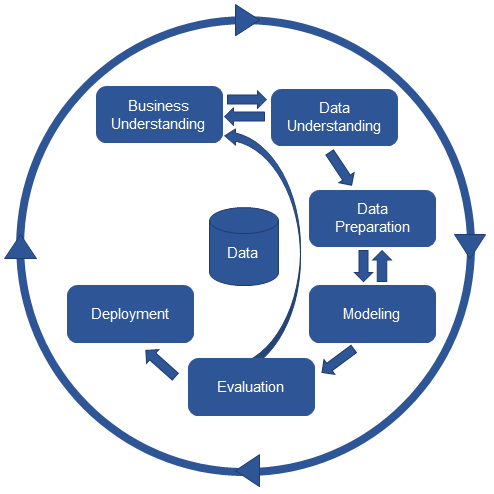
\includegraphics[width=0.8\linewidth]{Chapters/img/crisp_dm.png}
    \caption{Complete CRISP-DM Approach.}
    \label{fig:crisp_dm}
\end{figure}

In the following, we outline each phase briefly:
\begin{itemize}
\item Business Understanding\\
This initial phase focuses on understanding the project objectives and requirements from a
business perspective, and then converting this knowledge into a data mining problem
definition, and a preliminary project plan designed to achieve the objectives.
\item  Data Understanding\\
The data understanding phase starts with an initial data collection and proceeds with activities
in order to get familiar with the data, to identify data quality problems, to discover first
insights into the data, or to detect interesting subsets to form hypotheses for hidden
information.
There is a close link between Business Understanding and Data Understanding. The
formulation of the data mining problem and the project plan require at least some
understanding of the available data.
\item  Data Preparation\\
The data preparation phase covers all activities to construct the final dataset (data that will be
fed into the modeling tool(s)) from the initial raw data. Data preparation tasks are likely to be
performed multiple times, and not in any prescribed order. Tasks include table, record, and attribute selection, data cleaning, construction of new attributes, and transformation of data for
modeling tools.
\item Modeling\\
In this phase, various modeling techniques are selected and applied, and their parameters are
calibrated to optimal values. Typically, there are several techniques for the same data mining
problem type. Some techniques require specific data formats.
There is a close link between Data Preparation and Modeling. Often, one realizes data
problems while modeling or one gets ideas for constructing new data.
\item Evaluation
At this stage in the project you have built one or more models that appear to have high quality,
from a data analysis perspective. Before proceeding to final deployment of the model, it is
important to more thoroughly evaluate the model, and review the steps executed to construct
the model, to be certain it properly achieves the business objectives. A key objective is to
determine if there is some important business issue that has not been sufficiently considered.
At the end of this phase, a decision on the use of the data mining results should be reached.
\item Deployment\\
Creation of the model is generally not the end of the project. Usually, the knowledge gained
will need to be organized and presented in a way that the customer can use it. Depending on
the requirements, the deployment phase can be as simple as generating a report or as complex
as implementing a repeatable data mining process. In many cases it will be the user, not the
data analyst, who will carry out the deployment steps. In any case, it is important to
understand up front what actions will need to be carried out in order to actually make use of
the created models.
\end{itemize}


% section introduction (end)

\section{Business Understanding} % (fold)
\label{sub:business_understanding}

In the fishing industry it is necessary that vessels have licenses to use fishing techniques.
The problem is that there is a probability that vessels are using fishing techniques or gear that are not licensed to do so.
The objective is to classify the VMS data by fishing type. 
In this way we can try to confirm if each boat is carrying out the type of fishing for which it has the license payed.



% section business_understanding (end)


\section{Data Understanding} % (fold)
\label{sub:data_understanding}

The data we use for this objective is the same VMS Records as used in chapter 4 and VMS Vessels explained in chapter 3.2.
Let us focus on the use of speed, but not discriminating any of the remaining columns a prior without determining its potential in the contribution to a solution

% section data_understanding (end)



\section{Data Preparation} % (fold)
\label{sub:data_preparation}
To use data mining models, we need a dataset with all the data needed to feed the models. So, I created a dataset from VMS Vessels and VMS Records to end with Table \ref{table:vms_dataset}. 

\begin {table}[H]
\begin{center}
\begin{tabular}{c|c|c|c}
\textbf{Name }    & \textbf{Description} & \textbf{From} & \textbf{Why} \\
\hline
ID                & Key              & Native               & Identify the row           \\
VesselID          & Vessel Identifier   & VMS Records                & Identify the vessel  \\
UTC         & Date Time & VMS Records &Identify the time of the entry\\
LAT        & Latitude & VMS Records & Discriminated by fishing areas\\
LON        & Longitude & VMS Records & Discriminated by fishing areas\\
COG        & Direction & VMS Records & Course Over Ground\\
SOG        & Velocity & VMS Records & Discriminated by fishing velocity\\
LOA        & Length Overall & VMS Vessels & Discriminated by vessel type\\
GT        &  Gross Tonnage & VMS Vessels & Discriminated by vessel type\\
HP         &Vessel Power & VMS Vessels & Discriminated by vessel type\\
License        & Vessel's Linceses & VMS Vessels & Objective\\
           
\label{table:vms_dataset}
\end{tabular}
\caption {VMS Dataset}
\end{center}
\end {table}

The License that occurs in the dataset are:
\begin{itemize}
\item	Armadilhas / De abrigo / Alcatruzes
\item	Arrasto / De fundo de portas
\item	Arrasto / De fundo de portas / Crustáceos
\item	Arrasto / Pelágico / Com portas
\item	Cerco / para bordo / Tipo americano
\item	Emalhar de 1 pano / De deriva / Grandes Pelágicos
\item	Emalhar de 1 pano / De fundo
\item	Pesca à linha / Cana e linha de mão
\item	Pesca à linha / Palangre de fundo / Espécies demersais
\item	Pesca à linha / Palangre de Fundo + Cana e linha de mão
\item	Pesca à linha / Palangre de superfície / Grandes Migradores
\item	Tresmalho / De fundo
\end{itemize}


The first thing to test is the correlation of the data to check if licenses are strongly correlated to some of the other variables. In Figure \ref{fig:data_coor1} (the method used to find correlation was Pearson Correlation \cite{Benesty2009} that measures the degree of correlation and the direction of this correlation - whether positive or negative) between two metric scale variables). We can see that we can’t use the data as it is because de correlation between License and sog are very weak so we need to do some pre-processing.
\begin{figure}[H]
    \centering
    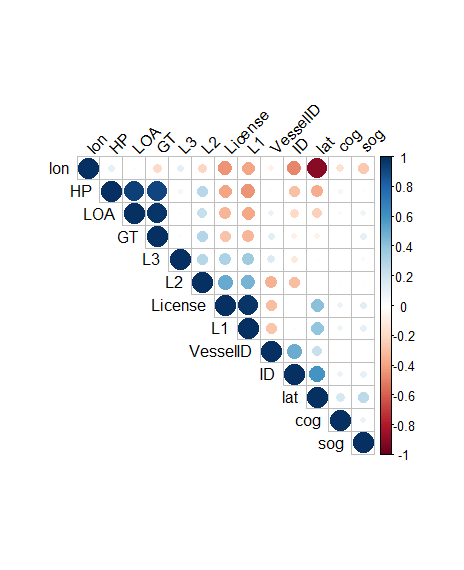
\includegraphics[width=0.8\linewidth]{Chapters/img/data_coor1.png}
    \caption{Data Correlation}
    \label{fig:data_coor1}
\end{figure}


The best way to achieve greater correlation between fishing speeds and licenses was the transformation of data to storage fishing average, maximum and minimum per day per vessel. This way it presents the results shown in Figure \ref{fig:data_coor2}.

\begin{figure}[H]
    \centering
    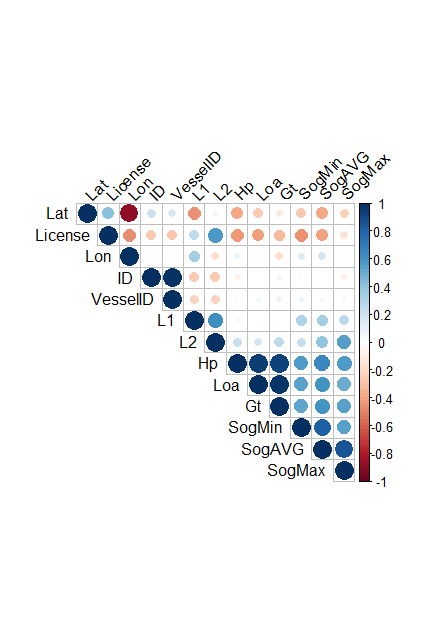
\includegraphics[width=0.8\linewidth]{Chapters/img/data_coor2.png}
    \caption{Data coorelation after preprocessing}
    \label{fig:data_coor2}
\end{figure}

The method used to transform the data consists of the following steps:
\begin{itemize}
\item	Create dataset in which data is grouped per day, per vessel.
\item	Use DSALib to get the minimum and maximum speeds of fishing for poop vessel. With this data, filter the dataset to be only with data in which the speed of the vessel is between the minimum and maximum obtained.

\end{itemize}

With this data we can also observe that the correlation between the license and the HP data (vessel power), Loa (Boat length) Gt (vessel weight) are quite significant. This is normal as different fishing activities require specific types of vessels. This does not mean that the type of vessel is only capable of entering a type of fishing activity.
For these reasons I will not use these variables in the model so as not to create a problem with bias.
\\
Regarding location data, used clustering techniques to discretize the data.
First, we need to know what the best number of clusters is. For that we used the same technique used in chapter 4.3 with the output in Figure \ref{fig:elbow_method_server}. The data used was the dataset filtered so we have only the positions of fishing. The chosen number of clusters was 4.

\begin{figure}[H]
    \centering
    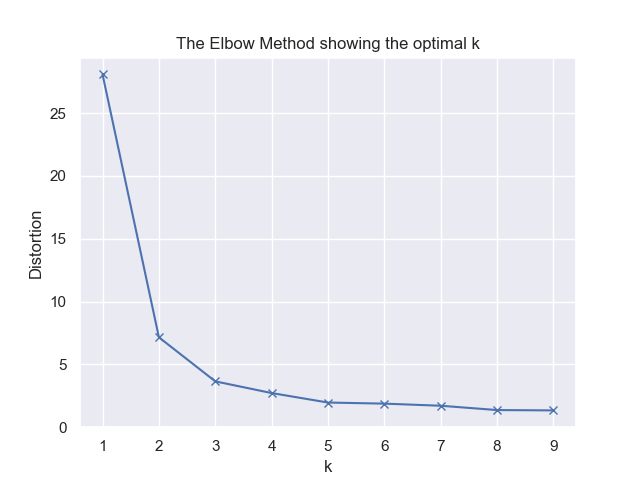
\includegraphics[width=0.8\linewidth]{Chapters/img/elbow_method_server.png}
    \caption{The elbow method showing the optinal k}
    \label{fig:elbow_method_server}
\end{figure}
Now we can create data mining models with location and velocity parameters.


% section data_preparation (end)

\section{Modeling} % (fold)
\label{sub:modeling}
Several data mining algorithms were used to create the necessary models to classify the license type with the VMS data.
\begin{itemize}
\item \textbf{ KMeans:} This model was used in the previous step with the GPS data, so it was classified in well-defined clusters in order to improve the operation of the data mining algorithms. The operation of this algorithm is described in chapter 4.3.

\item \textbf{ DecisionTrees: }
While in data mining a decision tree is a predictive model which can be used to represent both classifiers and regression models, in operations research decision trees refer to a hierarchical model of decisions and their consequences. The decision maker employs decision trees to identify the strategy which will most likely reach its goal. When a decision tree is used for classification tasks, it is most commonly referred to as a classification tree. When it is used for regression tasks, it is called a regression tree \cite{Rokach2014}.
Algorithms for constructing decision trees usually work top-down, by choosing a variable at each step that best splits the set of items \cite{ApplicationsReviews}.

\item \textbf{Neural Network: }
\item \textbf{Support Vector Machine: }
\end{itemize}

Cross \textendash validation \cite{CrossValidatory} provides a simple and effective method for both model selection and performance evaluation, widely employed by the machine learning community. Under k \textendash fold cross \textendash validation the data are randomly partitioned to form k disjoint subsets of approximately equal size. In the ith fold of the cross-validation procedure, the ith subset is used to estimate the generalization performance of a model trained on the remaining k \textendash 1 subsets. The average of the generalization performance observed over all k folds provides an estimate (with a slightly pessimistic bias) of the generalization performance of a model trained on the entire sample.
The k used to test this models is 10.




% section modeling (end)

\section{Evaluation} % (fold)
\label{sub:evaluation}
The model's test results are:

\begin{itemize}
\item \textbf{ DecisionTrees: }

\begin {table}[H]
\begin{center}
\begin{tabular}{c|c|c}
\textbf{Algorithm }    & \textbf{Gini} & \textbf{Entropy}  \\
\hline
Velocity and locations     & 0.7771544              & 0.7780856                \\
Velocity          & 0.7264879   & 0.730252            \\    
\label{table:cross_val_decision_trees}
\end{tabular}
\caption {Cross-Validation results for Decision Trees models}
\end{center}
\end {table}

\item \textbf{Neural Network: }

\begin {table}[H]
\begin{center}
\begin{tabular}{c|c|c|c|c}
\textbf{Layers }    & \textbf{15} & \textbf{30\* 3}& \textbf{100\* 3}  & \textbf{500\* 4}\\
\hline
Velocity and locations   & 0.6820688  & 0.7032381    &0.733293&     0.7433809      \\
Velocity               & 0.6614556   & 0.7178236      &0.7214212 &   0.7295752   \\    
\label{table:cross_val_nn}
\end{tabular}
\caption {Cross-Validation results for Neural Network models}
\end{center}
\end {table}

\item \textbf{Support Vector Machine: }
\begin {table}[H]
\begin{center}
\begin{tabular}{c|c|c|c}
\textbf{Kernel coefficient }    & \textbf{auto} & \textbf{scale} & \textbf{linearSVC} \\
\hline
Velocity and locations     & 0.6970205        & 0.694583            &0.601798\\
Velocity                   & 0.6610622   & 0.664224  &   0.5191799\\
\label{table:cross_val_svm}
\end{tabular}
\caption {Cross-Validation results for Support Vector Machine models}
\end{center}
\end {table}

\end{itemize}

Evaluate Results
Assessment of Data
Mining Results w.r.t.
Business Success
Criteria
Approved Models


Review Process
Review of Process

Determine Next Steps
List of Possible Actions
Decision

% section evaluation (end)


\section{Deployment} % (fold)
\label{sub:deployment}
Plan Deployment
Deployment Plan

Plan Monitoring and
Maintenance
Monitoring and
Maintenance Plan

Produce Final Report
Final Report
Final Presentation

Review Project
Experience
Documentation
% section deployment (end)

% chapter server (end)



